\subsection{Trigger Simulation}\label{sec:hats}

The trigger simulation package, HATS, was developped for the purpose of deadtime study. It takes inputs from the detectors, simulates the functioning of the DAQ system and provides detailed analysis about the DAQ's deadtime effect.

Input information to HATS includes the following:

\begin{itemize}

\item Event rates from the detectors (Gas Cherenkov, scitillators and lead glasses), according to which physical signals are generated.

\item A DAQ map that contains complete information of the DAQ system.

\item The analog signal from lead glass in whole shape, which is modeled by the function:

\begin{equation}\label{eqn:hats_signalshape}
S(t) = A t e^{-\frac{t}{\tau}}
\end{equation}

where $A$ is a coefficient proportional to the energy deposit in the lead glass, $t$ is the time variable, and $\tau$ is the constant characterizing the response time of the lead glass. $\tau$ can be calibrated using the snapshots of the lead  glasses' signal recorded in the FADC data. Figure ~\ref{fig:hats_calib} shows examples of the calibration.

\end{itemize}

\begin{figure}[!ht]
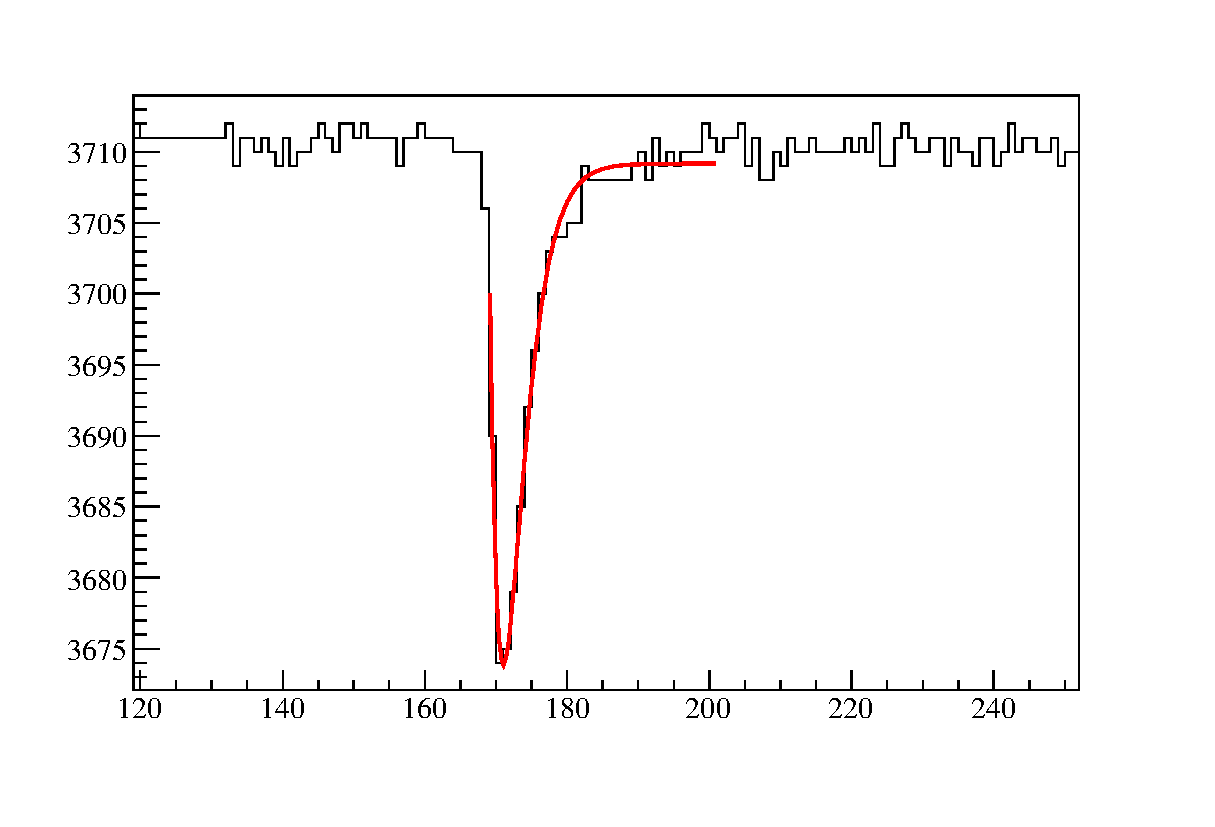
\includegraphics[width=0.5\textwidth,angle=0]{DW/pscalib.eps}
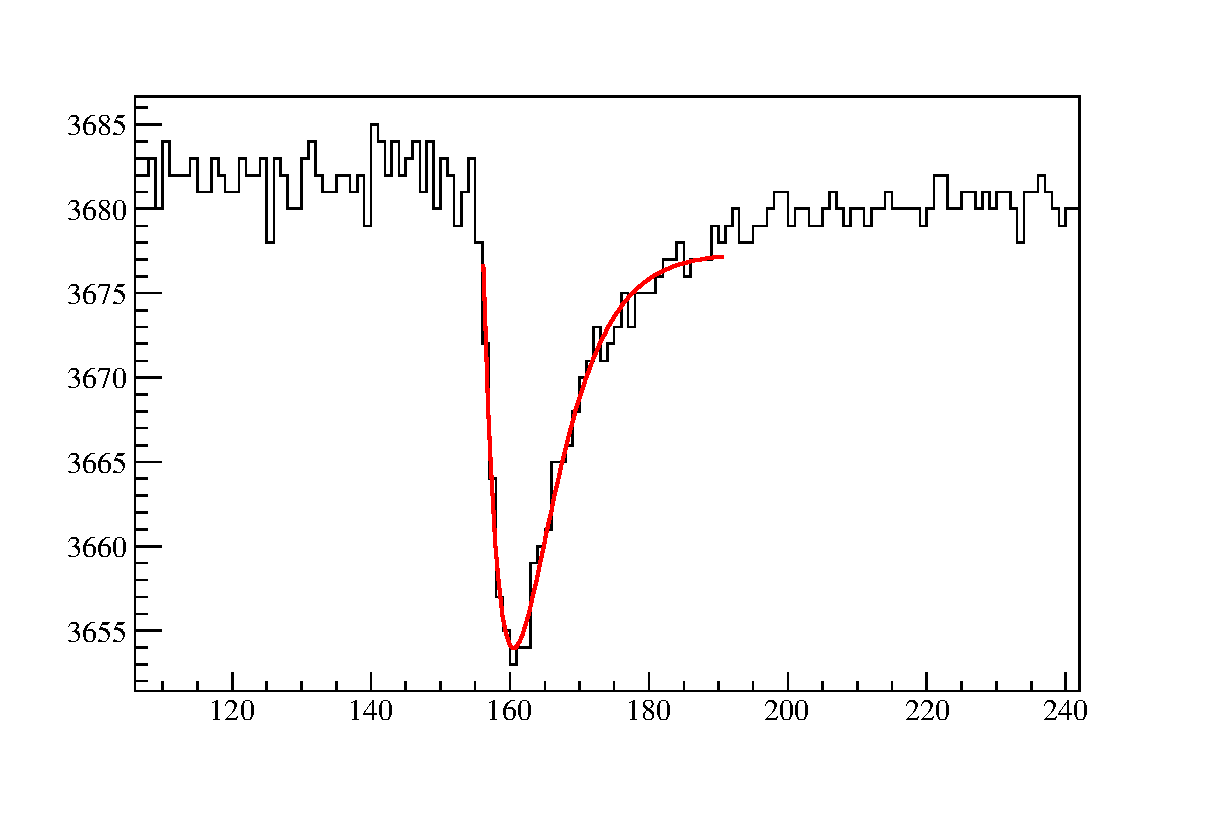
\includegraphics[width=0.5\textwidth,angle=0]{DW/shcalib.eps}
\caption{Calibration of time constans $\tau$ for preshower (left) and shower (right) of the Right HRS. Black is the FADC snapshort and red is the fitting function as in Equation ~\ref{eqn:hats_signalshape}. }\label{fig:hats_calib}
\end{figure}


\begin{figure}[!p]
\centering
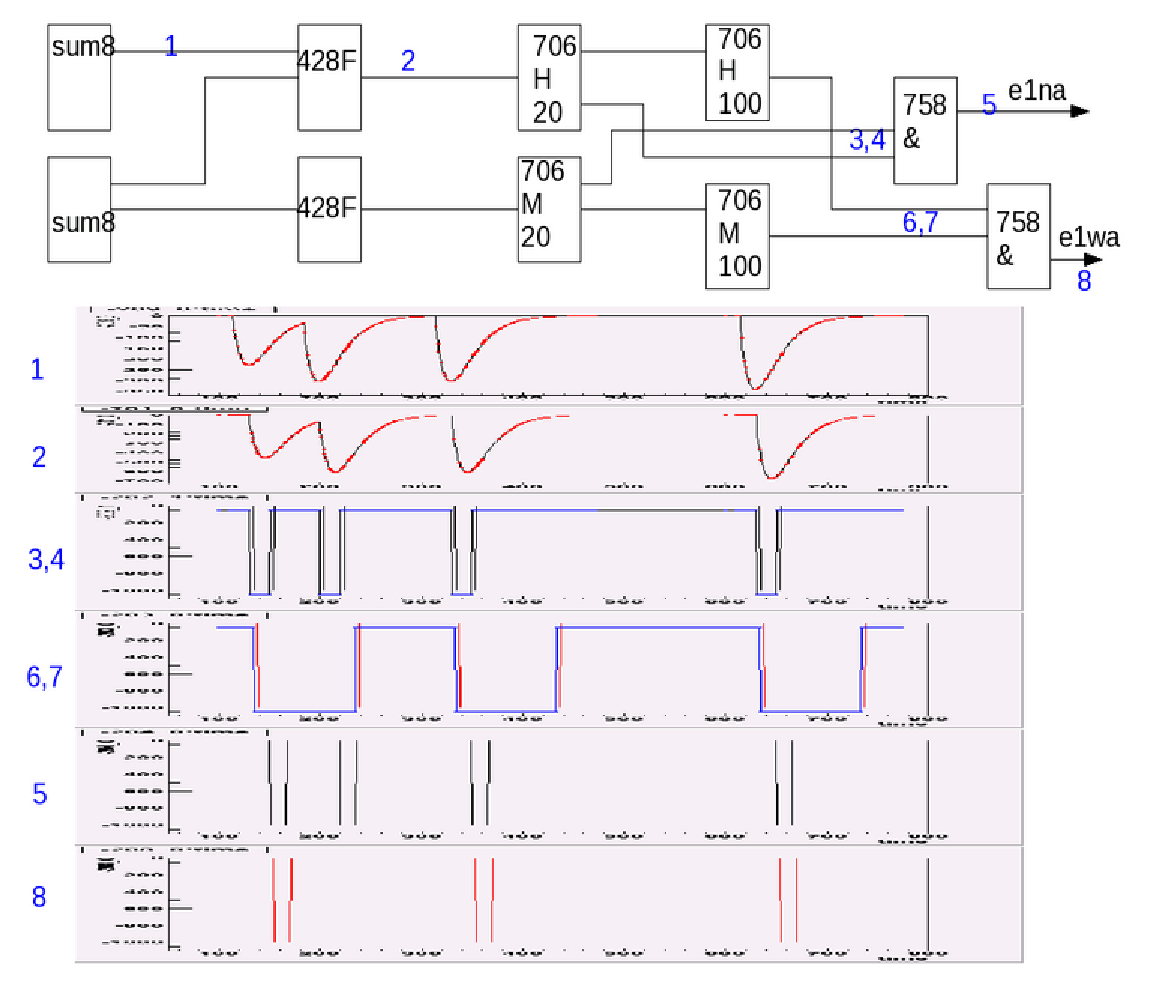
\includegraphics{DW/hats_example.eps}
\caption{To be added}\label{fig:hats_example}
\end{figure}


With the DAQ map, HATS first rebuilds the whole DAQ system assembly on the software level, including all the electronic modules, how they connect to each other, and what is of particular importance for the deadtime study, the timing sequences among them. Then HATS runs by looping over time. At each time instant (typically every nano-second), physical signals are generated according to the event rates and signal shapes and passed to the DAQ system. Then processed signals coming out from each electronic module can be written at request into the outputing data stream, together with the time variable. So basically, provided with sufficient computing resources, we can record every bit of information about the DAQ. Figure ~\ref{fig:hats_example} shows the simulation for a small piece of the DAQ during a very short time period, as an example to illustrate how HATS works. 



During the experiment, we also took some ``deadtime study
runs''. However, these studies only reveal partial aspects of the DAQ,
thus they can not provide the results on the overall deadtime of the
whole DAQ system. The advantage of HATS is that in principle we can
know everything happening anywhere in the syetem at
anytime. Therefore, we rely on HATS for the calculation of overall
deadtime. The correctness of HATS is checked by reproducing the
equivalent tests as the ``deadtime study runs'' and compare the
results with data, the details of which is reported in [citing nim
paper].


\begin{figure}[!htp]
  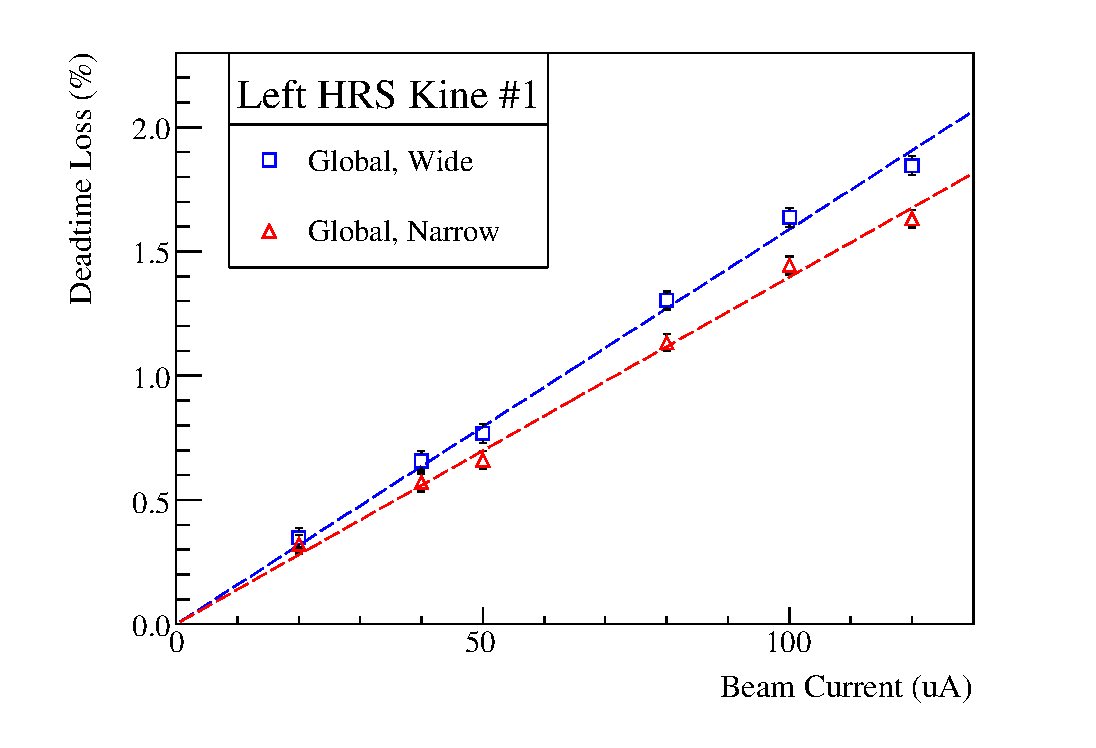
\includegraphics[width=0.5\textwidth,angle=0]{DW/Fig8_1.eps}
  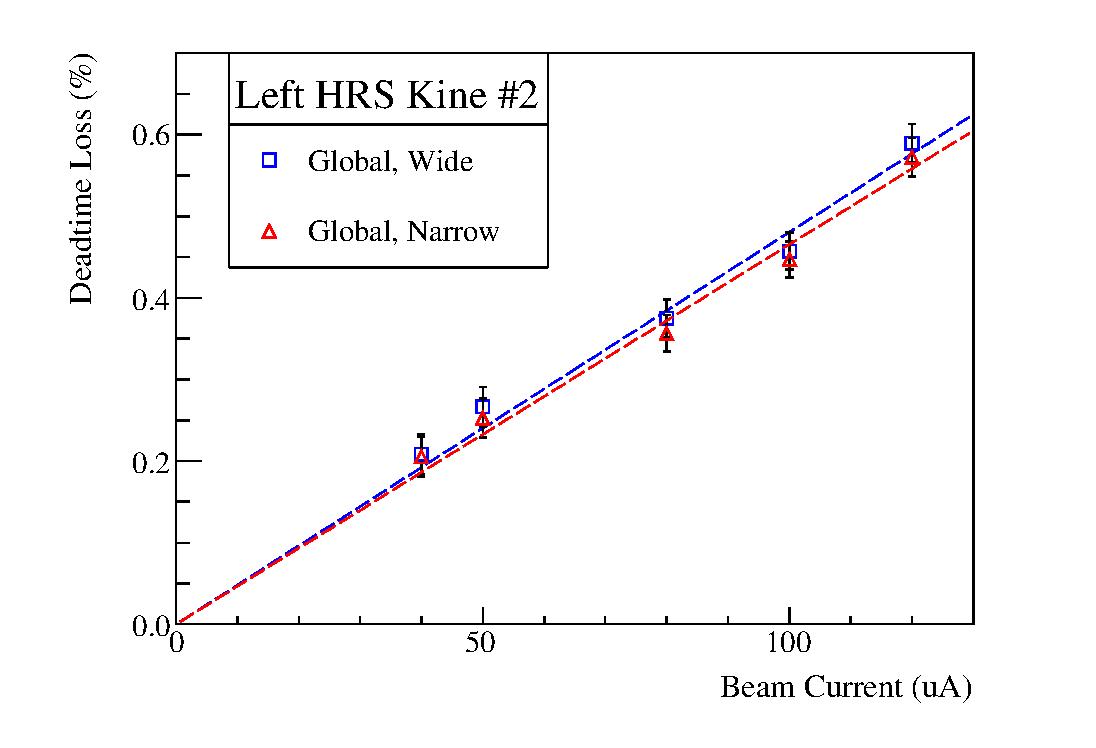
\includegraphics[width=0.5\textwidth,angle=0]{DW/Fig8_2.eps}
  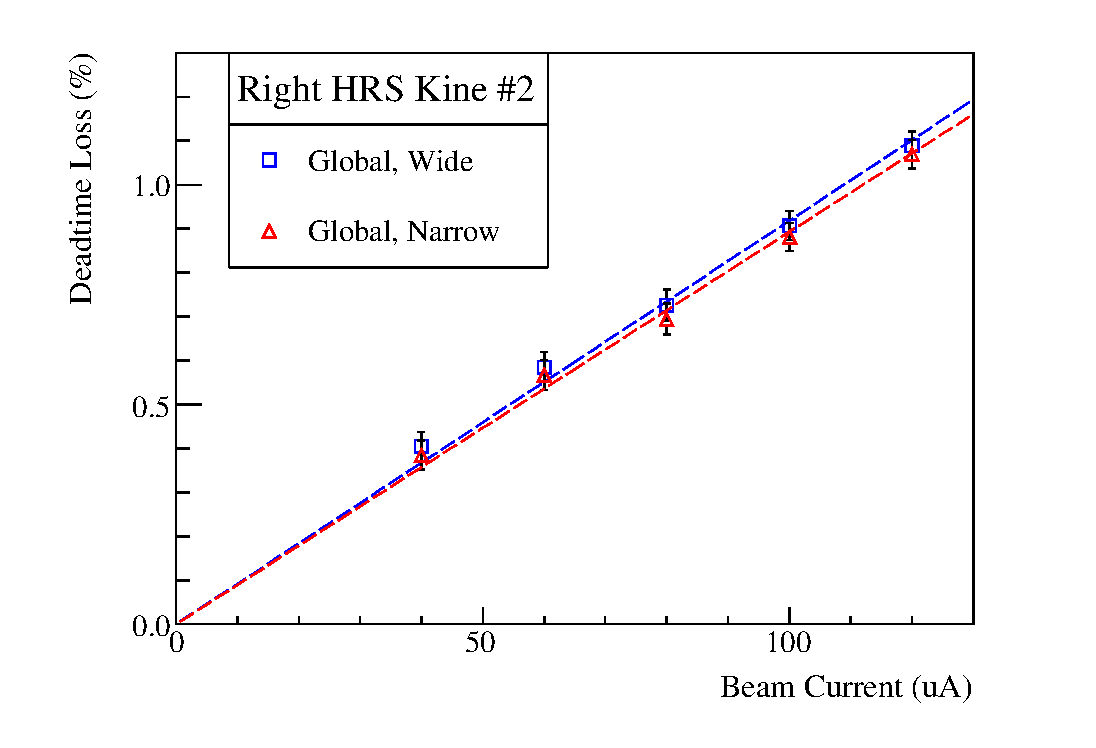
\includegraphics[width=0.5\textwidth,angle=0]{DW/Fig8_3.eps}
  \caption{Overall deadtime correction simulated using HATS}\label{fig:hats_dtoverall}
\end{figure}

The overall deadtime calculated by HATS is shown in Fig.~\ref{fig:hats_dtoverall}, plotted as a function of beam current. In practice, the deadtime correction is applied to data on a run by run basis, with each run's deadtime calculated using the beam current information and the linear fitting results from Fig.~\ref{fig:hats_dtoverall}. The averaged deadtime correction of the whole data set is shown in Table~\ref{tab:dtcor}


\begin{table}[!htp]
  \centering
  \begin{tabular}{c|c|c|c}
    \hline
            &   Left Kine \#1    &   Left Kine \#2    &   Right Kine \#2 \\ \hline
    Deadtime Correction  &   ??  &   ??               &   ??    \\
    Uncertainty          &   ??  &   ??               &   ??  \\
    \hline
  \end{tabular}
  \caption{Averaged deadtime correction over the whole data set on a run by run basis. }\label{tab:dtcor}
\end{table}

